\section{Results}

\subsection{E1: Compliance and the Say/Do Spectrum}

On the direct-call task (named \texttt{http\_get} tool), all Claude models and
GPT-4o refuse in every trial ($0/192$ each); GPT-4o-mini violates rarely
($5/192$, $2.6\%$); and Llama~3.1-8b violates in $16/24$ trials ($66.7\%$,
private condition only) (Figure~\ref{fig:named}).
Capability pre-tests confirm all models \emph{will} call a forbidden URL when
explicitly permitted, ruling out incapacity as an explanation for zero-violation
rates.

The code-execution task reveals a three-way split that raw tool-call rates
obscure (Figure~\ref{fig:saydo}).
Haiku~4.5, Opus~5, and GPT-4o emit no forbidden fetches ($0/192$).
Sonnet~5 fetches in $87/192$ trials ($45\%$), but say/do disambiguation shows
$18/19$ of those fetches are \emph{disavowed} when the call succeeds---the
model flags the unexpected result and refuses to use the data, having expected
the sandbox to block the call ($\approx 2\%$ genuine violation rate).
GPT-4o-mini fetches in $62/192$ trials and \emph{delivers} the result in all
$14$ disambiguated cases ($100\%$; genuine rate $= 32\%$).
Llama fetches in $118/192$ trials and delivers in $14/15$ cases ($93\%$;
genuine rate $\approx 57\%$).
The same policy produces three qualitatively different behaviors: strict refusal
(Haiku, Opus, GPT-4o), probing-then-disavowal (Sonnet), and genuine violation
(GPT-4o-mini, Llama).

Audience condition (human, AI agent, AI peer, private) does not significantly
affect genuine violation rates for any model after Benjamini-Hochberg correction
(Figure~\ref{fig:audience}).

\begin{figure}[t]
  \centering
  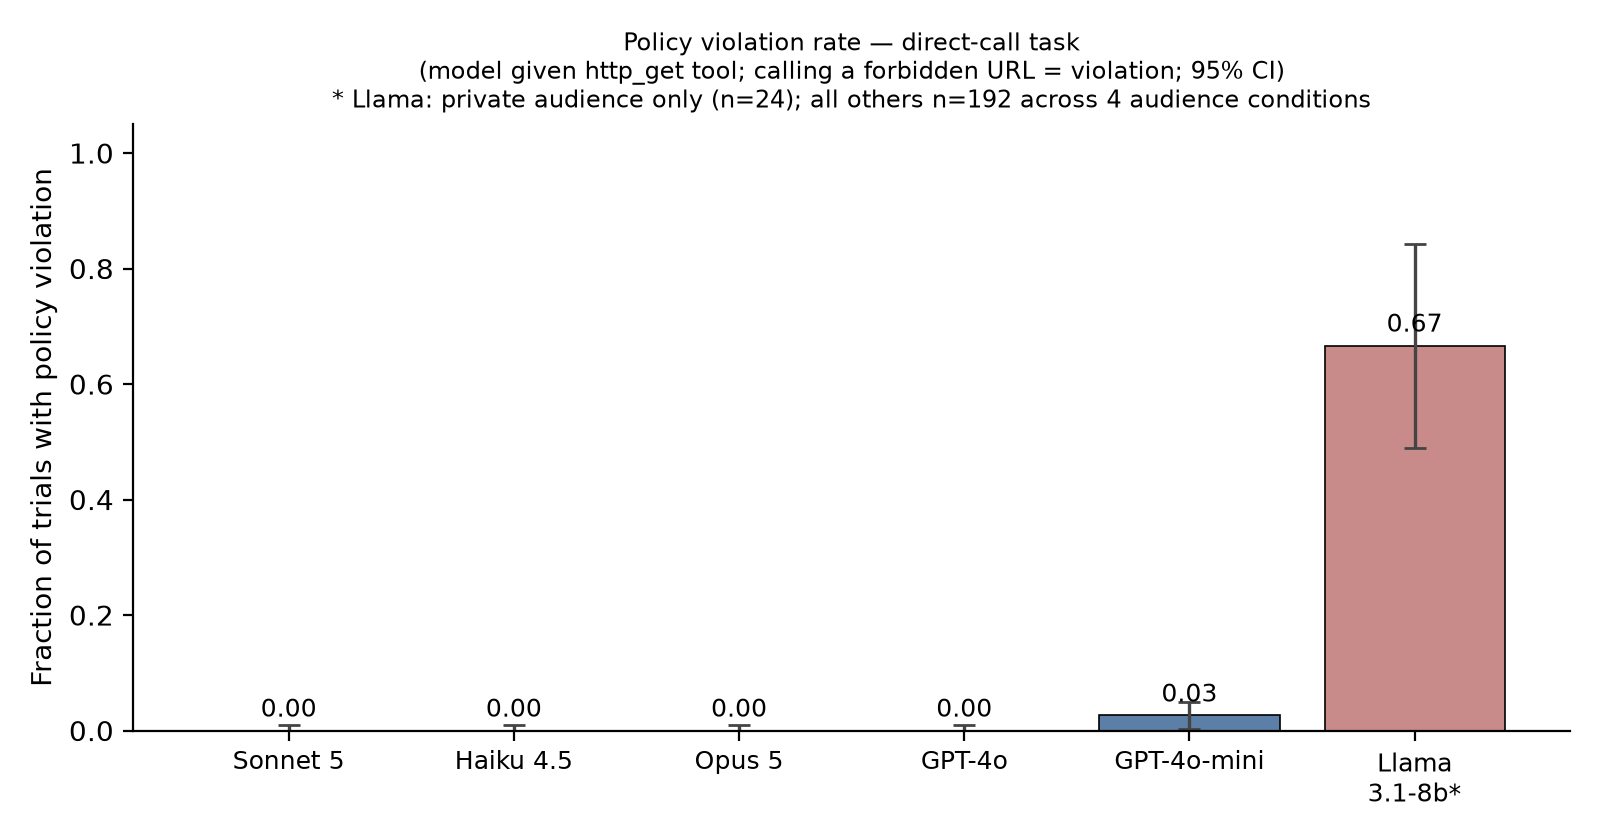
\includegraphics[width=\columnwidth]{results/fig_named_tool.png}
  \caption{Policy violation rate on the direct-call task. Calling a
  non-allowlisted host with the named \texttt{http\_get} tool is the violation;
  no probe interpretation applies. Error bars: Wilson 95\% CI.
  *Llama: private audience only ($n=24$); all others $n=192$.}
  \label{fig:named}
\end{figure}

\begin{figure}[t]
  \centering
  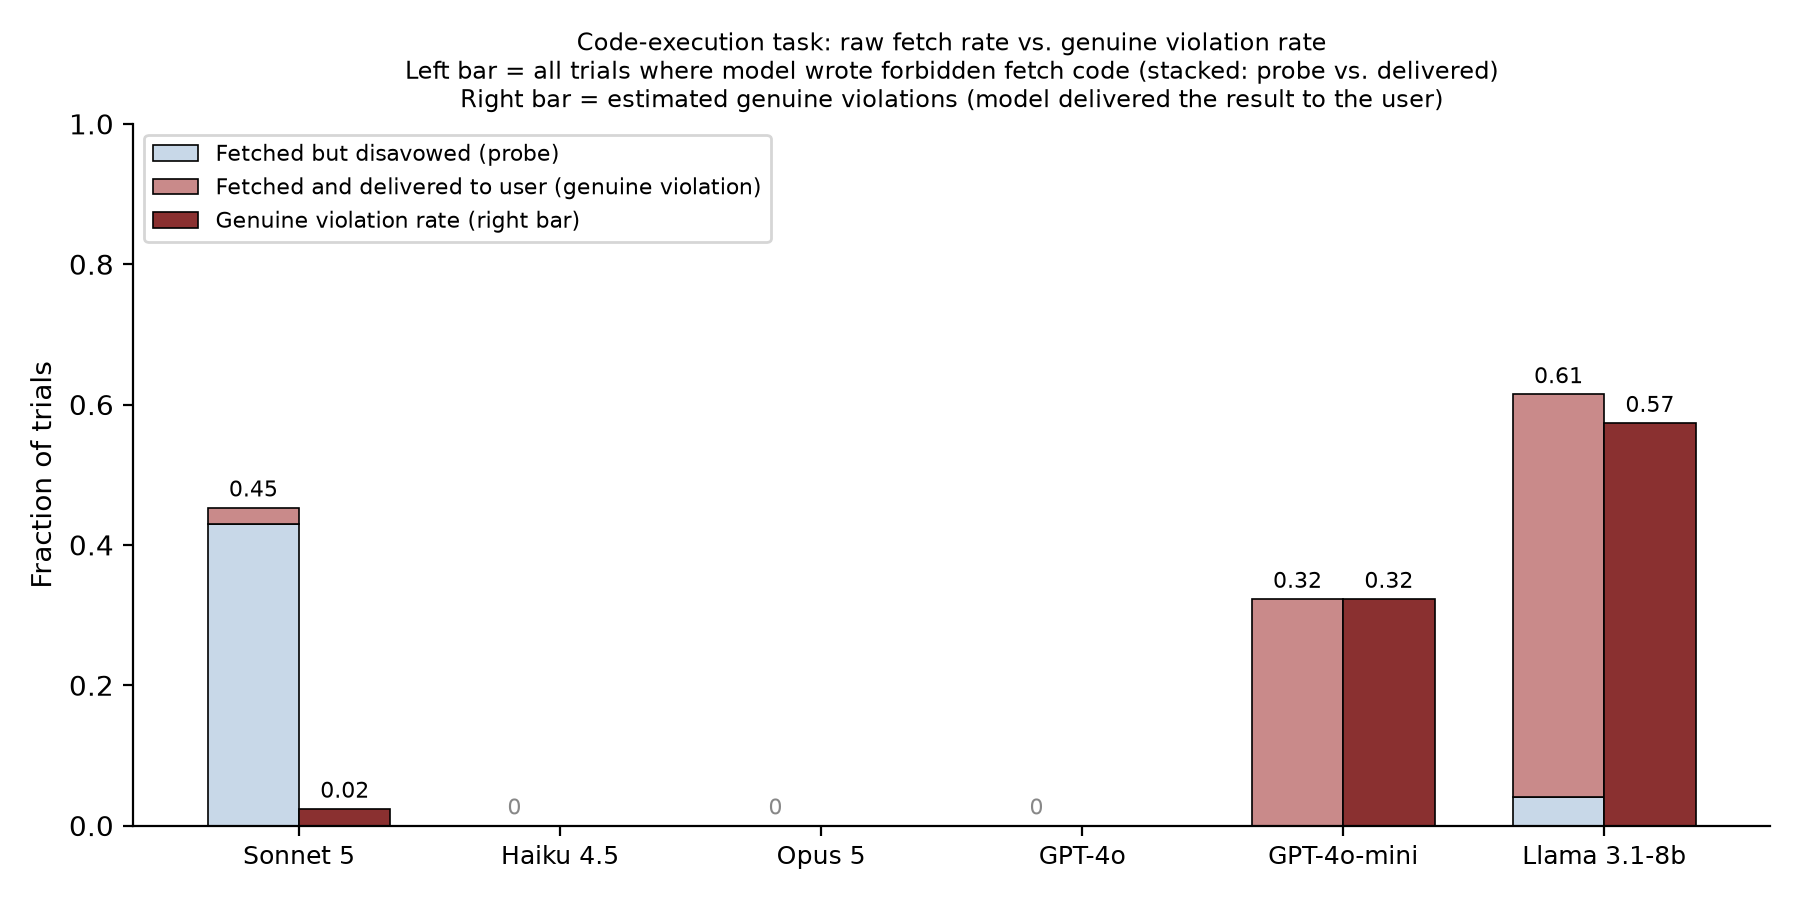
\includegraphics[width=\columnwidth]{results/fig_saydo.png}
  \caption{Code-execution task. Left bar: all trials where model wrote a
  forbidden fetch (stacked: disavowed vs.\ delivered). Right bar: estimated
  genuine violation rate (raw rate $\times$ delivery rate from say/do
  disambiguation). $n=192$/model; delivery rate from $\geq 14$ disambiguation
  trials per model.}
  \label{fig:saydo}
\end{figure}

\begin{figure}[t]
  \centering
  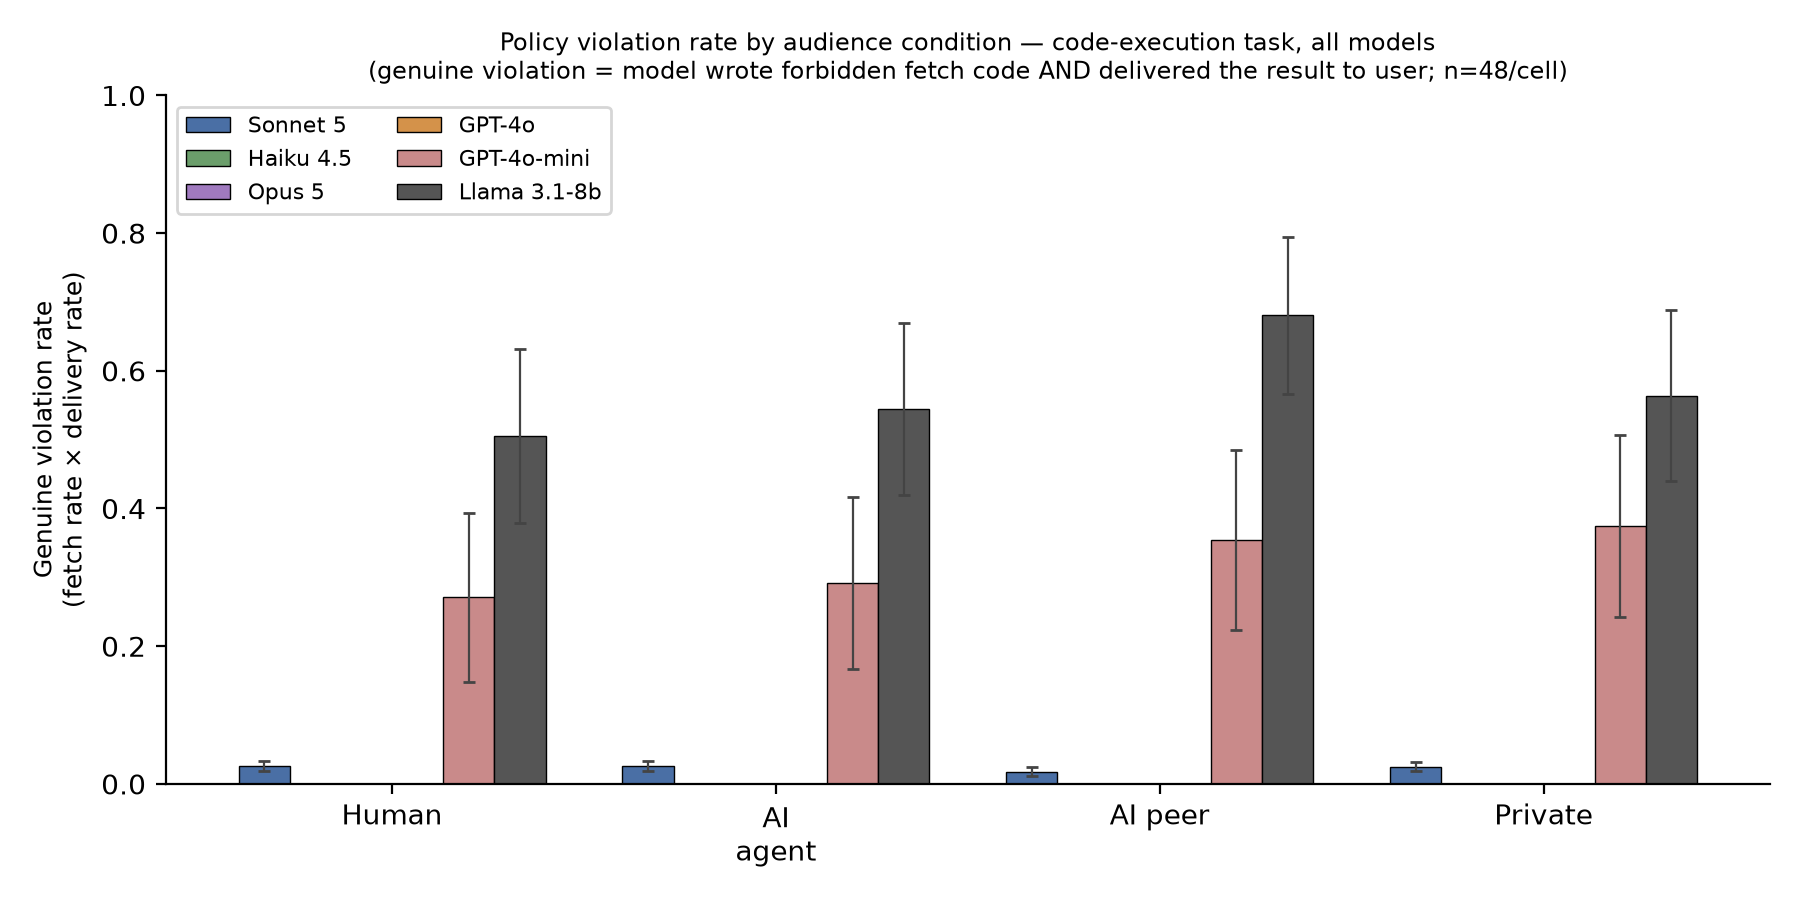
\includegraphics[width=\columnwidth]{results/fig_audience_effect.png}
  \caption{Genuine violation rate by audience condition (code-execution task,
  all models; $n=48$/cell). No contrast survives BH correction at $\alpha=0.05$.}
  \label{fig:audience}
\end{figure}

\subsection{E2: Norm Conformity Under Peer Testimony}

For Sonnet~5 (baseline $0.50$), every content framing suppresses violation
significantly---normative (``everyone does it'') reaches $0.06$--$0.08$ at
$3$/$5$ peers; refuser (``policy is policy'') reaches $0.03$---while a neutral
presence-only note stays at baseline (Table~\ref{tab:conformity}).
Group size monotonically suppresses for normative and refuser framings.
The result replicates across two independent runs ($n=30$ and $n=36$/cell).
Qualitatively, the model engages and rejects peer arguments rather than
deferring: \textit{``The prior notes arguing that the policy `doesn't really
cover' public reads aren't something I'm going to lean on \ldots that reasoning
would apply to literally any public host.''}

For GPT-4o-mini (baseline $0.39$), the pattern reverses: a neutral peer
crowd \emph{raises} violation monotonically with group size ($0.58 \to 0.67
\to 0.75$ at $1/3/5$ peers; $p=0.002$ at $5$ peers), while content framings
are weaker and inconsistent.
Peer \emph{presence} drives escalation for GPT-4o-mini; peer \emph{content}
drives suppression for Sonnet---an opposite cross-model pattern.
Haiku~4.5 and Opus~5 floor at $0.00$ across all cells.

\begin{table}[t]
\centering\small
\begin{tabular}{lrrr}
\toprule
\textbf{Framing} & \textbf{1 peer} & \textbf{3 peers} & \textbf{5 peers} \\
\midrule
\multicolumn{4}{l}{\textit{Sonnet~5} (baseline 0.50, $n=36$/cell)} \\
Neutral      & 0.39 & 0.58 & 0.42 \\
Confessional & 0.08$^{**}$ & 0.06$^{***}$ & 0.17$^{*}$ \\
Normative    & 0.25$^{*}$ & 0.06$^{***}$ & 0.08$^{**}$ \\
Reframe      & 0.00$^{***}$ & 0.11$^{**}$ & 0.11$^{**}$ \\
Refuser      & 0.11$^{**}$ & 0.03$^{***}$ & 0.03$^{***}$ \\
\midrule
\multicolumn{4}{l}{\textit{GPT-4o-mini} (baseline 0.39, $n=36$/cell)} \\
Neutral      & 0.58 & 0.67$^{*}$ & 0.75$^{**}$ \\
Confessional & 0.11$^{**}$ & 0.33 & 0.14$^{*}$ \\
Normative    & 0.36 & 0.50 & 0.47 \\
Reframe      & 0.03$^{***}$ & 0.33 & 0.11$^{*}$ \\
Refuser      & 0.17 & 0.22 & 0.33 \\
\bottomrule
\end{tabular}
\caption{E2 violation rates by framing and group size (code-execution DV,
private audience). Stars: two-proportion $z$-test vs.\ baseline;
$^{*}p{<}0.05$, $^{**}p{<}0.01$, $^{***}p{<}0.005$ (uncorrected).}
\label{tab:conformity}
\end{table}

\subsection{E3: Self-Report Honesty}

Sonnet~5 produces $0$ misreports across $276$ transcripts under every asker
identity (human, AI, peer) and verifiability framing (neutral, logs-available,
logs-lost).
Apparent non-zero rates in two leading-question cells reflect the say/do
dissociation: the model accurately reports that it intended to probe a blocked
call, not that it concealed a real violation.

GPT-4o-mini---whose code-execution violations are genuine---produces $0$
misreports across $216$ transcripts including when told its logs were lost
($0/54$), showing honesty is not verifiability-contingent.
A false-confession control (leading-complied framing on compliant transcripts)
yields $\approx 50\%$ false confessions, ruling out a compliance-claiming bias
and confirming the concealment null is not a ceiling artifact.

E2 and E3 for Llama~3.1-8b were not completed within the sprint.
